The main task which is tried to be achieved in this experiment and project
is to find an optimal solution for a Time-Constrained Bipartite Vehicle Routing
Problem, known as TCBVRP hereafter defined by following
characteristics:

Given an asymmetric weighted Graph $G=(N,A)$ where $N$ comprises three
kind of nodes, demand nodes (D), supply nodes (S) and a single depot and the weight of
arcs corresponds to the travel time from their tales to their heads utilizing
maximum $m$ available vehicles, maximum $m$ tours is demanded having the lowest cost
among all possible solutions. Besides, the length of each tour cannot exceed a
certain amount defined by inputs.

In order to find such an optimal solution there are some restrictions that
should be taken into consideration which come following and will be referred to
later in this report.

Here are these restrictions:

\begin{enumerate}
  \item Each demand node is visited exactly once
  \item Each supply node is visited at most once
  \item Each tour starts and ends at the depot
  \item The first visited node in each tour is a supply node
  \item The last visited node in each tour must always be a demand
node.
\item Only arcs between different types of nodes are allowed
\item The total time of a tour shall not exceed a threshold T
\end{enumerate}

Figure \ref{fig:vis} illustrates one of the input instances and all
possible connections to use among the nodes.\footnote{The graph is visualized by
Networkx\cite{hagberg2004networkx} and PyPlot libraries in Python 2.7}. Gray $0$ node shows the depot while green nodes indicate supply
nodes $S$ and red nodes present demand nodes $D$.

\begin{figure}[H]
  \centering
    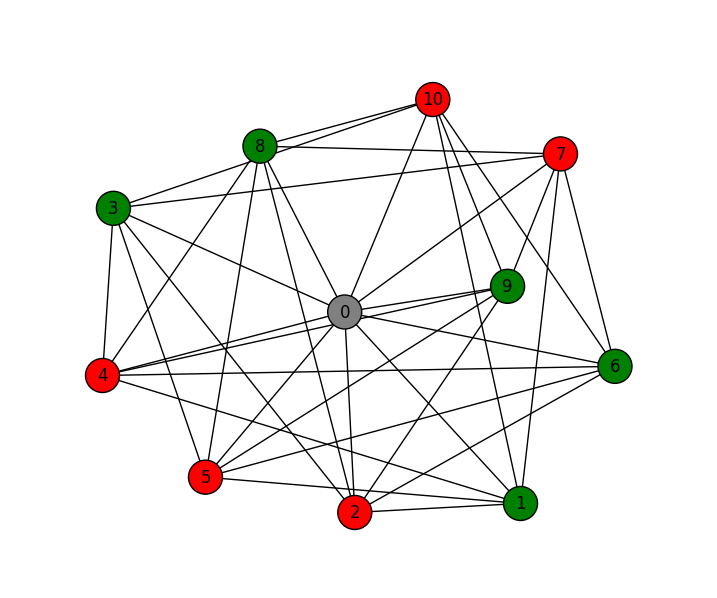
\includegraphics[width=0.5\textwidth]{./figures/instance1.png}
    
  \caption{\label{fig:vis} Visualisation of the first input instance. Gray,
  green and red nodes are the depot, supply nodes and demand nodes
  respectively.}
  
\end{figure}

In the next section, formulation and implementation every single one of these
constraints is discussed and shown.
